\documentclass[a4paper, 12pt]{report}
\usepackage{cmap}
\usepackage{amssymb}
\usepackage{amsmath}
\usepackage{graphicx}
\usepackage{amsthm}
\usepackage{upgreek}
\usepackage{setspace}
\usepackage{mathtools}
\setcounter{secnumdepth}{5}
\setcounter{tocdepth}{5}
\numberwithin{equation}{section}
\renewcommand{\theequation}{\arabic{equation}}
\usepackage[T2A]{fontenc}
\usepackage[utf8]{inputenc}
\usepackage[normalem]{ulem}
\usepackage{mathtext} % русские буквы в формулах
\usepackage[left=2cm,right=2cm, top=2cm,bottom=2cm,bindingoffset=0cm]{geometry}
\usepackage[english,russian]{babel}
\usepackage[unicode]{hyperref}
\newenvironment{Proof} % имя окружения
{\par\noindent{$\blacklozenge$}} % команды для \begin
{\hfill$\scriptstyle\square$}
\newcommand{\Rm}{\mathbb{R}}
\newcommand{\Cm}{\mathbb{C}}
\newcommand{\Z}{\mathbb{Z}}
\newcommand{\I}{\mathbb{I}}
\newcommand{\N}{\mathbb{N}}
\newcommand{\rank}{\operatorname{rank}}
\newcommand{\Ra}{\Rightarrow}
\newcommand{\ra}{\rightarrow}
\newcommand{\FI}{\Phi}
\newcommand{\Sp}{\text{Sp}}
\newcommand{\ol}{\overline}

\renewcommand{\leq}{\leqslant}
\renewcommand{\geq}{\geqslant}

\renewcommand{\alpha}{\upalpha}
\renewcommand{\beta}{\upbeta}
\renewcommand{\gamma}{\upgamma}
\renewcommand{\delta}{\updelta}
\renewcommand{\varphi}{\upvarphi}
\renewcommand{\phi}{\upvarphi}
\renewcommand{\tau}{\uptau}
\renewcommand{\theta}{\uptheta}
\renewcommand{\eta}{\upeta}
\renewcommand{\lambda}{\uplambda}
\renewcommand{\sigma}{\upsigma}
\renewcommand{\psi}{\uppsi}
\renewcommand{\mu}{\upmu}
\renewcommand{\omega}{\upomega}
\renewcommand{\xi}{\upxi}
\renewcommand{\epsilon}{\upvarepsilon}
\renewcommand{\rho}{\uprho}
\renewcommand{\varepsilon}{\upvarepsilon}

\renewcommand{\d}{\partial}
\renewcommand{\Re}{\operatorname{Re}}
\newcommand{\const}{\operatorname{const}}
\newcommand{\intx}{\int\limits_{x_0}^x}
\newcommand\Norm[1]{\left\| #1 \right\|}
\newcommand{\sumk}{\sum\limits_{k=0}^\infty}
\newcommand{\sumi}{\sum\limits_{i=0}^\infty}
\newtheorem*{theorem}{Теорема}
\newtheorem*{cor}{Следствие}
\newtheorem*{lem}{Лемма}
\title{\textbf{\Huge{Численные методы математической физики}}\\Конспект по 4 курсу 
	специальности «прикладная математика»\\(лектор А. М. Будник)}
\date{}
\begin{document}
	\maketitle
	\tableofcontents{}
	\newpage
	\section*{Введение.}
	В данном курсе мы будем рассматривать задачи математической физики в частных производных. Основной принцип решения состоит в том, что дифференциальное уравнение мы заменяем разностным и ищем приближенное решение на сетке узлов. Такой способ называется \textit{методом конечных разностей} (\textit{методом сеток}). А раздел численных методов, посвященный теории метода конечных разностей, носит название \textit{теория разностных схем}. 
	\\\\
	Выделим два основных момента при решении:
	\begin{enumerate}
		\item построение дискретных разностных аппроксимаций для уравнений математической физики и исследование основных характеристик этих аппроксимаций: погрешности, устойчивости и точности разностных схем;
		\item решение разностных уравнений прямыми или итерационными методами, которые выбираются из соображений экономичности вычислительного алгоритма.
	\end{enumerate}
	\chapter{Способы построения и исследования разностных схем.}
	\section{Сетки и сеточные функции.}
	При численном решении той или иной математической задачи мы не можем воспроизвести приближенное решение для всех значений аргумента. Поэтому в области задания функции выбирается конечное множество точек, и приближенное решение задачи ищется в этих точках.
	\\\\
	$\bullet$ \textit{Это множество называется \textbf{сеткой}, а отдельные точки этого множества -- \textbf{узлами сетки}.}
	\\\\
	$\bullet$ \textit{Функция, определенная в узлах сетки, называется \textbf{сеточной функцией}.}
	\\\\
	Заменяя области непрерывного изменения аргумента сеткой, то есть областью дискретного изменения аргумента, мы осуществляем аппроксимацию пространства решения дифференциального уравнения пространством сеточной функции.
	\\\\
	\textbf{Пример сетки на отрезке (одномерный случай).}\\\\
	В качестве области определения искомой функции мы рассматриваем отрезок на оси $x$.
	\begin{enumerate}
		\item \textbf{Равномерная сетка.}
		Не ограничивая общности, возьмем отрезок $[0,1]$ и разобьем его на $N$ равных частей точками $$x_0=0,\ x_1,\ \ldots,\ x_{N-1},\ x_N=1.$$
		Расстояние между соседними точками назовем \textit{шагом сетки} и обозначим его через $h$, а точки $x_i$ примем в качестве \textit{узлов сетки}, $i=\overline{0,N}$. Тогда множество всех $x_i$ составляют \textit{равномерную сетку} на отрезке $[0,1]$, которую будем обозначать следующим образом
		$$\overline \omega _ h = \left\{x_i = ih,\ i=\overline{0, N},\ h = \dfrac1N\right\}.$$
		\textit{Множество граничных узлов} обозначим как $$\gamma_h = \{x_0, x_N\}.$$
		А все остальные точки образуют \textit{множество внутренних узлов}
		$$ \omega _ h = \left\{x_i = ih,\ i=\overline{1, N-1},\ h = \dfrac1N\right\}.$$
		Таким образом, можно записать 
		$$\overline \omega _h = \omega _h \cup \gamma _h.$$
		\item \textbf{Неравномерная сетка.}
		Возьмем отрезок $[0,1]$ и разобьем его на $N$ частей точками $$0=x_0 < x_1 <\ldots< x_{N-1} < x_N=1.$$
		Тогда мы можем записать неравномерную сетку с граничными узлами 
		$$\hat {\overline \omega} _ h = \left\{x_i,\ i=\overline{0, N},\ x_0 = 0, \ x_N=1\right\}.$$
		Шаг неравномерной сетки зависит от номера узла и удовлетворяет условию нормировки $$\sum_{i=1}^{N} h_i=1,\ \text{где } h_i=x_i - x_{i-1}.$$
		Аналогично случаю равномерной сетки можно записать $$\hat {\overline \omega} _ h = \hat \omega_h \cup \hat\gamma _h.$$
	\end{enumerate}
	\textbf{Пример сетки на плоскости (двумерный случай).}
	\begin{enumerate}
		\item \textbf{Прямоугольник.} Исходная область прямоугольника $$\overline G = \{(x_1, x_2),\ 0\leq x_\alpha \leq l_\alpha,\ \alpha=1,2\}$$
		$$
	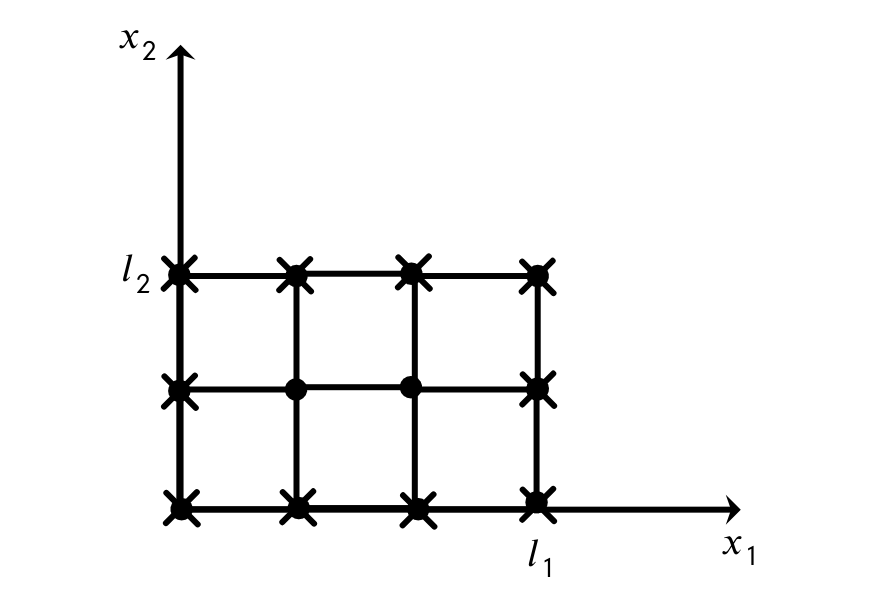
\includegraphics[scale=0.5]{images/img_1}
		$$
		(кружочками обозначены внутренние узлы, а крестиками -- внешние).\\\\
		Сначала построим равномерную сетку. Разобьем отрезки $[0, l_\alpha]$ на $N_\alpha$ частей точками $$0 = x_{\alpha,0} < x_{\alpha, 1} < \ldots < x_{\alpha, N_\alpha -1} < x_{\alpha, N_\alpha} = l_\alpha.$$ Через точки деления проводим прямые, параллельные координатной оси. В качестве узлов двумерной сетки возьмем точки пересечения этих прямых. Общее количество узлов сетки равно $(N_1+1) \times (N_2 + 1)$, а их распределение характеризуется векторным параметром $$h = \{h_{\alpha,1},\ldots, h_{\alpha, N_\alpha},\ h_{\alpha, i_\alpha} = x_{\alpha, i_\alpha} - x_{\alpha, i_\alpha-1},\ i_\alpha = \overline{1, N_\alpha}, \alpha=1,2\}.$$
		Тогда \textit{неравномерную двумерную сетку} можно обозначить
		$$\hat{ \overline \omega} _ h = \hat{ \overline \omega}_{h_1, h_2} = \hat{ \overline \omega} _ {h_1} \times \hat{ \overline \omega} _ {h_2} = \{(x_{1,i_1}, x_{2, i_2}),\ i_\alpha = \overline{0, N_\alpha},\ x_{\alpha, 0} = 0, x_{\alpha, N_\alpha } = l_\alpha,\ \alpha=1,2\}.$$
		Если по каждому направлению шаги сетки равны между собой, то мы получим \textit{двумерную равномерную сетку}
		$${ \overline \omega} _ h = { \overline \omega}_{h_1, h_2} = \hat{ \overline \omega} _ {h_1} \times \hat{ \overline \omega} _ {h_2} = \left\{(x_{1,i_1}, x_{2, i_2}),\ x_{\alpha, i_\alpha} = i_\alpha h_\alpha,\ i = \overline{0, N_\alpha},\ h_\alpha=\frac{l_\alpha}{N_\alpha},\ \alpha=1,2\right\}.$$
		\item \textbf{Область сложной формы.} Пусть нам дана область нерегулярной (сложной) формы $\overline G = G \cup \Gamma$. Для построения сетки мы заключим эту область в прямоугольник $[a,b]\times [c,d]$. В этом прямоугольнике мы строим прямоугольную сетку. Для простоты зададим прямоугольную равномерную сетку. 
		$$
			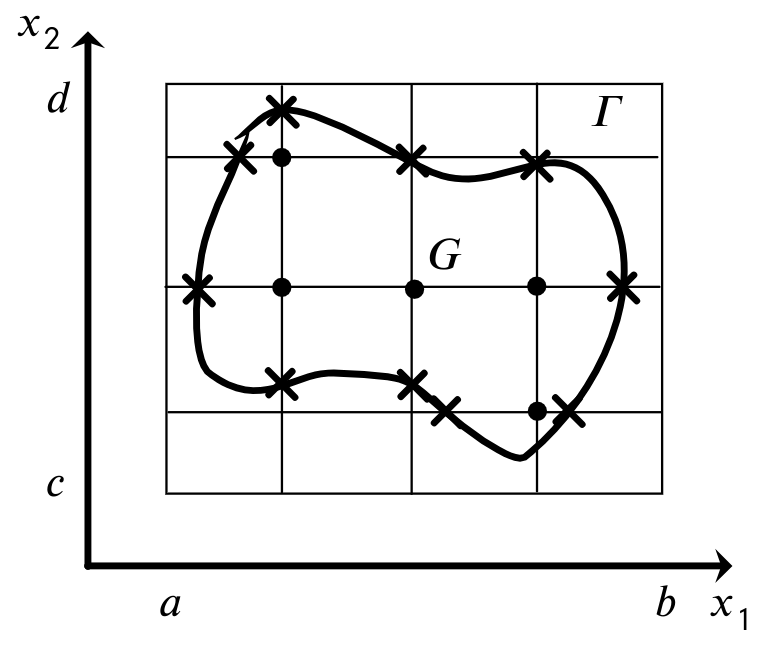
\includegraphics[scale=0.5]{images/img_2}
		$$
		Те узлы, которые попали внутрь этой сетки, будем считать \textit{внутренними}, обозначим их совокупность $\omega _h$. Точки пересечения прямых $x_\alpha = i_\alpha l_\alpha$, $\alpha=1,2$ с границей $\Gamma$ назовем \textit{граничными узлами}, обозначим их совокупность $\gamma_h$. Тогда сеткой будет множество узлов $$\overline \omega_h = \omega_h \cup \gamma_h$$
		Если исходная сетка в прямоугольнике $[a,b]\times [c,d]$ является равномерной, то сетка $\overline\omega_h$ в области $\overline G$ является неравномерной.\\\\
	\end{enumerate}
	\textbf{Замечания.}
	\begin{enumerate}
		\item Аналогичным образом строятся сетки и большей размерности. 
		\item В зависимости от геометрии исходной области можно использовать и другие ортогональные системы координат.
		\item Кроме прямоугольных сеток можно строить, так называемые, треугольные сетки, элементарными ячейками которой являются треугольники. 
	\end{enumerate}
	Пусть $u(x)$ --- это функция непрерывного аргумента $x = (x_1, \ldots, x_p)\in \overline G$ и $u(x) \in H_0$ ($H_0$ --- функциональное пространство). Если в области $\overline G$ введена сетка $\overline \omega_h$, то вместо функции $u(x)$ можно рассматривать функцию дискретного аргумента $y(x) = y_h$, где $x\in \ol \omega _h$, и эту функцию будем называть \textit{сеточной функцией}, значения которой вычисляются в узлах, а сама функция зависит от шага сетки $h$.\\\\
	Множество сеточных функций образует пространство $H_h$ -- \textit{пространство сеточных функций}. Следуя методу конечных разностей, мы заменяем пространство $H_0$ пространством $H_h$. Если $h$ -- параметр, то мы можем рассматривать множество сеточных пространств $\{H_h\}$ для каждого фиксированного $h$.\\\\
	Для того, чтобы оперировать функций, нам нужен аппарат для исследования функций и их сравнения. Мы рассматриваем линейные пространства, а для линейных пространств вводится понятие нормы. Соответственно мы определяем \textit{сеточный аналог нормы} $$\Norm {\cdot}_0 \sim \Norm {\cdot} _h.$$
	Например, если $H_ 0 = C[0,1]$, то в нем вводится норма $\Norm {\cdot}_0 = \underset{x\in [0,1]} {\max}|u(x)|$. Тогда сеточным аналогом может быть норма $$\Norm {\cdot}_h = \underset{x \in \ol \omega_h}{\max}|y(x)|.$$
	Если взять $H_ 0 = L_2[0,1]$, то в нем вводится норма $\Norm {\cdot}_0 = (u,u)^\frac12$. Тогда сеточным аналогом может быть норма $$\Norm {\cdot}_h = \left(\sum_{i=1}^{N-1}hy_i^2\right)^\frac12.$$
	Предположим, что функция $u(x)$ -- это решение некоторой дифференциальной задачи. Тогда $y_h(x)$ -- это решение приближенной, или разностной задачи. Для сравнения точного и приближенного решений сеточная функция доопределяется во всех точках области $\ol G$. В результате получается функция непрерывного аргумента $\widetilde{y}_h$, тогда точность решения может быть оценена как $$\Norm{\widetilde{y}_h - u}_0.$$
	Другой подход заключается в том, что мы исходное пространство $H_0$ отображаем в пространство $H_h$. Каждой функции $u(x)\in H_0$ ставится в соответствие сеточная функция $u_h(x), x \in \ol \omega _h$, при этом $u_h = P_h u \in H_h$, где $P_h$ -- это линейный оператор проектирования из $H_0$ в $H_h$. Тогда точность решения оценивается как $$\Norm{y-u_h}_h.$$ Для того, чтобы эта операция была корректна, естественно требовать, чтобы норма пространства $H_h$ аппроксимировала норму пространства $H_0$, то есть $$\lim\limits_{h\to 0}\Norm{u_h}_h = \Norm{u}_0.$$
	$\bullet$ \textit{Это требование называется \textbf{условием согласованности норм}.}\\\\
	\section{Разностная аппроксимация дифференциальных операторов.}
	\subsection{Локальная аппроксимация.}
	Пусть задан линейный дифференциальный оператор $L$ действующий на функцию $u=u(x)$. Для того, чтобы аппроксимировать (приближенное вычислить) его в любой точке $x\in \omega _h$ разностным оператором $L_h$, необходимо в начале указать или выбрать шаблон $\text {Ш} (x)$. \\\\
	$\bullet$ \textit{Под \textbf{шаблоном} $\text{Ш}(x)$ мы понимаем множество узлов сетки, которое будет использоваться при аппроксимации оператора $L$ оператором $L_h$ в точке $x$.}\\\\
	$\bullet$ \textit{П\textbf{огрешность аппроксимации дифференциального оператора $L$ разностным оператором $L_h$ в точке $x$} называется величина }
	\begin{equation}
		\psi(x) = L_hu(x) - Lu(x),\ x\in \omega_h.
	\end{equation}
	$\bullet$ \textit{Будем говорить, что \textbf{разностный оператор $L_h$ аппроксимирует дифференциальный оператор $L$ с порядком $m>0$ в точке $x$}, если можно представить} $$\psi(x) = O(h^m).$$
	Рассмотрим способ построения разностных операторов, получивший название \textit{метод неопределенных коэффициентов}. На выбранном шаблоне $\text{Ш}(x)$ разностную аппроксимацию будем искать в виде линейной комбинации значений функции в точках шаблона \begin{equation}
		L_hu(x) = \sum_{\xi \in \text{Ш}(x)} A_h(x, \xi) u(\xi).
	\end{equation}
	В формуле (2) $A_h(x, \xi)$ -- это неизвестные коэффициенты, выбранные таким образом, чтобы погрешность аппроксимации имела в точке $x$ заданный (чаще всего максимально возможный) порядок. Практический выбор значений коэффициентов осуществляется путем разложения погрешности аппроксимации в ряд Тейлора, то есть мы представляем $$\psi(x) = \sum_{\xi \in \text{Ш}(x)} A_h(x, \xi) u(\xi) - Lu(x),$$
	а затем раскладываем получившееся выражение в ряд Тейлора в окрестности точки $x$. После приведения мы получаем в итоге линейную комбинацию 
	$$\psi(x) = \sum_{\xi \in \text{Ш}(x)} A_h(x, \xi) u(\xi) - Lu(x) = \sum_{|j|\geq 0} B_h^{(j)}(x) u^{(j)}(x).$$
	После этого мы приравниваем к нулю максимально возможное количество первых членов этого разложения. Как правило, количество этих членов совпадает с количеством неизвестных коэффициентов. После этого, решив систему линейных уравнений, находим коэффициенты $A_h$ и по формуле (2) записываем искомый разностный оператор $L_h$.
	\\\\
	\textbf{Замечания.}
	\begin{enumerate}
		\item Выбор шаблона зависит от порядка производных, входящих в исходный операторов $L$, а также от требуемой точности аппроксимации.
		\item Легко видеть, что для аппроксимации дифференциального оператора, содержащего производную $k$-ого порядка по некоторой переменной, необходимо использовать шаблон, содержащий не менее $(k+1)$ точку вдоль координатного направления соответствующей переменной.
		\item Метод неопределенных коэффициентов является не единственным способом построения разностных операторов. Известен в литературе также метод \textit{численного дифференцирования}.
	\end{enumerate}
	\textbf{Примеры.}
	\begin{enumerate}
		\item Пусть задан дифференциальный оператор $$Lu(x) = \dfrac{d u(x)}{dx} = u'(x).$$
		\begin{enumerate}
			\item Пусть нам дан шаблон $\text{Ш}(x) = \{x, x+h\}$. Тогда по формуле (2) составляем линейную комбинацию
			$$u(x) = a_0 u(x) + a_1u(x+h).$$
			Записываем выражение для погрешности аппроксимации
			$$\psi(x)= a_0u(x) + a_1u(x+h) - u'(x).$$
			Затем производим разложение выражения в ряд Тейлора в окрестности точки $x$ и приводим подобные при значениях функции и ее производных
			$$\psi(x)= a_0u(x) + a_1u(x+h) - u'(x) = \underbrace{(a_0+a_1)}_{B ^{(0)}}u(x) + \underbrace{(ha_1 - 1)}_{B^{(1)}} u'(x) + \dfrac{h^2}{2} a_1 u''(x) + \ldots.$$
			Приравнивая коэффициенты $B^{(j)}$ к нулю, получаем систему линейных уравнений 
			$$\begin{cases}
				a_0+a_1 = 0,\\
				ha_1 - 1= 0.
			\end{cases}$$
			Тогда $$a_0 = -\dfrac 1h,\ a_1 = \dfrac 1h.$$
			Таким образом, мы построили разностный оператор вида 
			\begin{equation}
				L_hu(x) = \dfrac{u(x+h) - u(x)}{h} = u_x
			\end{equation}
			$\bullet$ \textit{Обозначение называется \textbf{правой разностной производной}.}\\\\
			При этом $$\psi(x) = \dfrac h2 u''(x) + \ldots = O(h),$$ то есть разностный оператор (3) аппроксимирует исходный оператор $L$ с первым порядком.\\\\
			$\bullet$ \textit{Величина $\dfrac h 2 u''(x)$ называется \textbf{главным членом погрешности аппроксимации}.}
			\item Пусть нам дан шаблон $\text{Ш}(x) = \{x-h, x\}$. Поступая аналогичным образом, мы можем построить оператор вида 
			\begin{equation}
				L_hu(x) = \dfrac{u(x) - u(x-h)}{h} = u_{\ol x}
			\end{equation}
			$\bullet$ \textit{Обозначение $u_{\ol x}$ называется \textbf{левой разностной производной}. }
			\\\\
			Легко видеть, что $$\psi(x) = -\dfrac h2 u''(x) + \ldots = O(h).$$ 
			\item Пусть нам дан шаблон $\text{Ш}(x) = \{x-h, x, x+h\}$. Проделав те же вычисления, мы получим выражение 
			\begin{equation}
				L_hu(x) = \dfrac{u(x+h) - u(x-h)}{2h} = u_{\circ x}
			\end{equation}
			$\bullet$ \textit{Обозначение $u_{\ol x}$ называется \textbf{центральной разностной производной}.}
			\\\\
			Легко видеть, что $$\psi(x) = -\dfrac {h^2}{6} u'''(x) + O(h^4) = O(h^2).$$ 
		\end{enumerate}
		Можно заметить, что с увеличением точек шаблона будет также увеличиваться погрешность аппроксимации.\\\\
		Можно построить однопараметрическое семейство операторов для аппроксимаиции первой производной следующего вида $$L_h^{(\sigma)}u(x) = \sigma u_x + (1-\sigma)u_{\ol x},$$
		где $\sigma$ -- это любое вещественное число. Выражение для погрешности имеет следующий вид
		$$\psi(x) = (2\sigma - 1)\dfrac h2 u''(x) + O(h^2).$$
		Очевидно, что при любом $\sigma \ne \frac 12$ разностный оператор будет иметь первый порядок аппроксимации $\psi(x) = O(h).$ Иначе мы получаем второй порядок аппроксимации $\psi(x) = O(h^2)$ , при этом легко видеть, что $$L_h^{(0,5)} = \dfrac 12(u_x + u_{\ol x}) = u_{\hat x}.$$
		\item Пусть нам дан дифференциальный оператор $$Lu(x) = u''(x).$$ Оператор второго порядка, поэтому для аппроксимации нужно как минимум 3 точки. Возьмем шаблон $\text{Ш}(x) = \{x-h, x, x+h\}$. Применяя метод неопределенных коэффициентов, мы получим следующий разностный оператор \begin{equation}
		L_h u(x) = \dfrac{u(x+h) - 2u(x) + u(x-h)}{h^2}=u_{\ol xx}
		\end{equation}
		$\bullet$ \textit{Обозначение $u_{\ol x x}$ называется \textbf{второй разностной производной}.}\\\\
		Погрешность будет иметь вид $$\psi(x) = \dfrac {h^2}{12} u^{IV}(x) + O(h^4) = O(h^2),$$ то есть имеет второй порядок, а не первый, как мы могли ожидать. Оказывается, что именно симметрия шаблона обеспечивает повышение порядка аппроксимации. Но на произвольной сетке мы получили бы первый порядок аппроксимации.\\\\
		\textbf{Замечания.}
		\begin{enumerate}
			\item Символы, используемые для обозначения разностных производных неслучайны, а является формальными операторами разностного дифференцирования и предписывают, как осуществлять аппроксимации. Например, если мы имеем разностный оператор $u_{\ol x x}$, то можно записать
			\begin{multline*}
				u_{\ol x x} = (u_{\ol x}(x))_x = \dfrac{u_{\ol x}(x+h) - u_{\ol x}(x)}{h} = \dfrac{1}{h}\left(\dfrac{u(x+h) - u(x)}{h} - \dfrac{u(x) - u(x-)}{h}\right) =\\= \dfrac{u(x+h) - 2u(x) - u(x-h)}{h^2}.
			\end{multline*}
			Можно также записывать $$u_{\ol x}(x+h) = u_x(x),\ \dfrac12 (u_x + u_{\ol x}) = u_{ \overset{\circ}{x}}.$$ Соответственно, мы можем конструировать разные операторы. Существуют также и разностные аналоги формул Грина.
			\item Разложение погрешности $\psi(x)$ по степеням $h$ можно использовать для повышения порядка аппроксимации. Например, мы можем заменить четвертую производную четвертой разностной производной в выражении $$u_{\ol x x}(x) - u''(x) = \dfrac{h^2}{12} u^{IV}(x) + O(h^4) = \dfrac{h^2}{12}\left(u_{\ol x x\ol x x}(x) + O(h^2)\right) + O(h^4).$$
			Тогда можно построить разностный оператор $$L_hu(x) = u_{\ol x x}(x) - \dfrac{h^2}{12} u_{\ol x x\ol x x}(x).$$
			Шаблон уже будет $$\text{Ш}(x) = \{x-2h, x-h, x, x+h, x+2h\},$$ а погрешность аппроксимации $$\psi(x) = O(h^4).$$
		\end{enumerate}
		\item Пусть дан дифференциальный оператор $$Lu = \dfrac{\d u}{\d t} - \dfrac{\d ^2 u}{\d x ^2},\ u=u(x,t),\ (x,t) \in \omega_{h\tau}.$$
		\begin{enumerate}
			\item Шаблон может иметь вид $$
				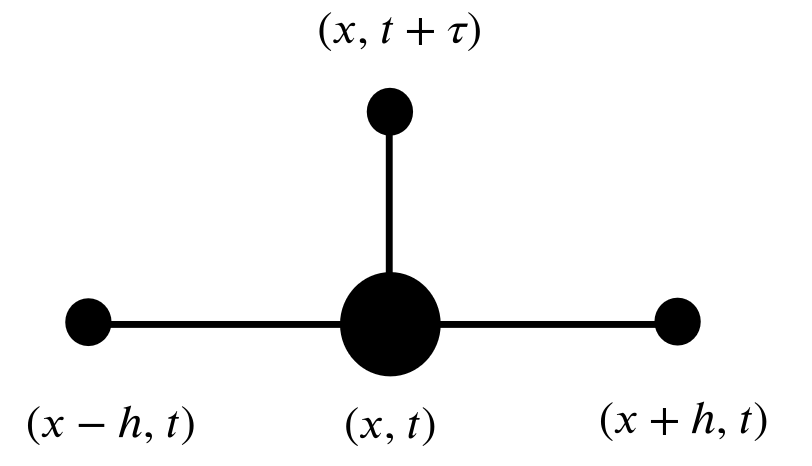
\includegraphics[scale=0.25]{images/img_3}$$
			\item Шаблон может иметь вид $$
			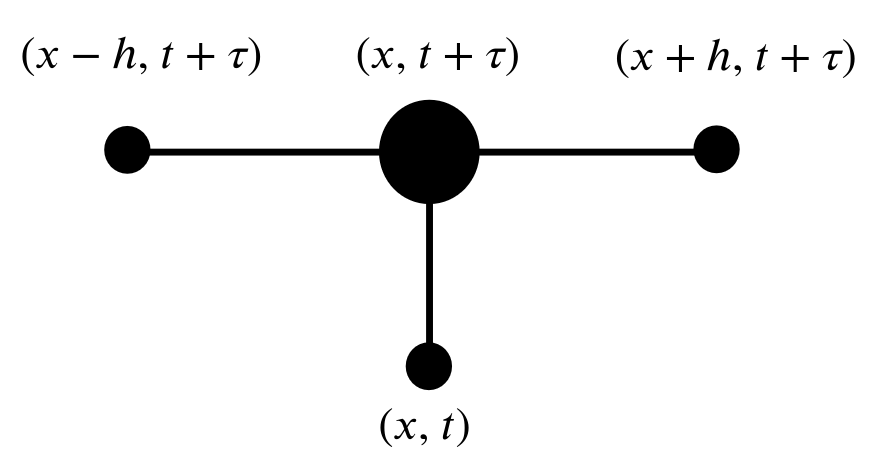
\includegraphics[scale=0.25]{images/img_4}
			$$
			\item Шаблон может иметь вид $$
				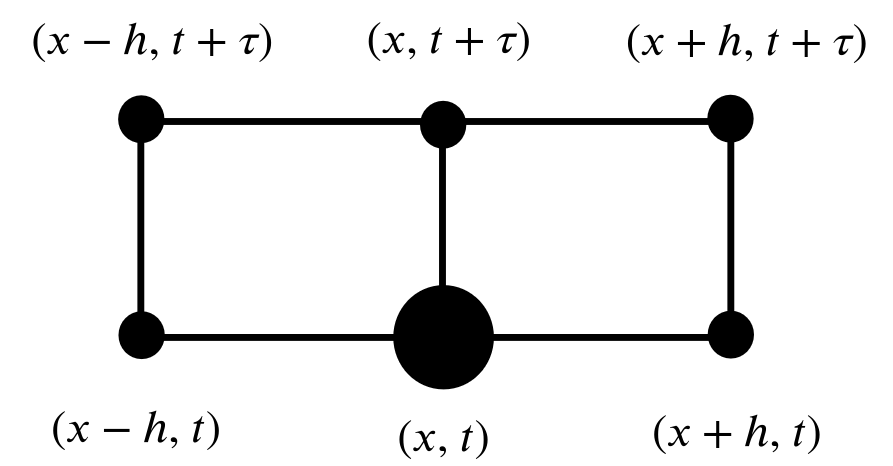
\includegraphics[scale=0.25]{images/img_5}
			$$
		\end{enumerate}
		Для шаблона (а) мы можем записать оператор $$L_{h\tau} u = \dfrac{u(x, t+\tau) - u(x,t)}{\tau} - \dfrac{u(x+h, t) - 2u(x,t) + u(x-h, t)}{h^2}.$$
		Такая форма записи называется \textit{индексной.}
		Учитывая введенные обозначения, мы можем записать этот оператор также в форме 
		\begin{equation}
			L_{h\tau} u = \dfrac{u(x, t+\tau) - u(x,t)}{\tau} - \dfrac{u(x+h, t) - 2u(x,t) + u(x-h, t)}{h^2} = u_t - u_{\ol x x}.
		\end{equation}
		Используем следующие обозначения: $$u(x,t) = u,\ u(x, t+\tau) = \hat u, \ u(x, t-\tau) = \check {u}.$$
		Тогда для случая (b) можно записать \begin{equation}
			L_{h\tau} u = u_t - \hat u_{\ol x x}.
		\end{equation}
		Для случая (c) мы можем построить однопараметрическое семейство аппроксимаций вида
		\begin{equation}
			L_{h\tau}^{(\sigma)}u = u_{\hat t} - (\sigma \hat u_{\ol x x} - (1-\sigma) u_{\ol x x}),\ \sigma \ne 0,\ \sigma \ne 1.
		\end{equation}
		Разностный оператор (9) аппроксимирует исходный дифференциальный оператор со вторым порядком по $x$ при любых $\sigma$ и первым порядком по $\tau$ при $\sigma =0, \sigma = 1$. Или вторым порядком по $\tau$ при $\sigma = \dfrac 12$. То есть можно записать записать 
		\begin{equation}
			\begin{cases}
				\psi(x,t) = O(\tau + h^2),\ \sigma \ne \dfrac 12,\\
				\psi(x,t) = O(\tau^2 + h^2),\ \sigma = \dfrac 12.
			\end{cases}
		\end{equation}
		\item Пусть дан дифференциальный оператор $$Lu = \dfrac{\d ^2u}{\d t^2} - \dfrac{\d ^2 u}{\d x^2}.$$
		Сейчас по каждому из направлений у нас будет по 3 точки.
		\begin{enumerate}
			\item Шаблон может иметь вид 
			$$
				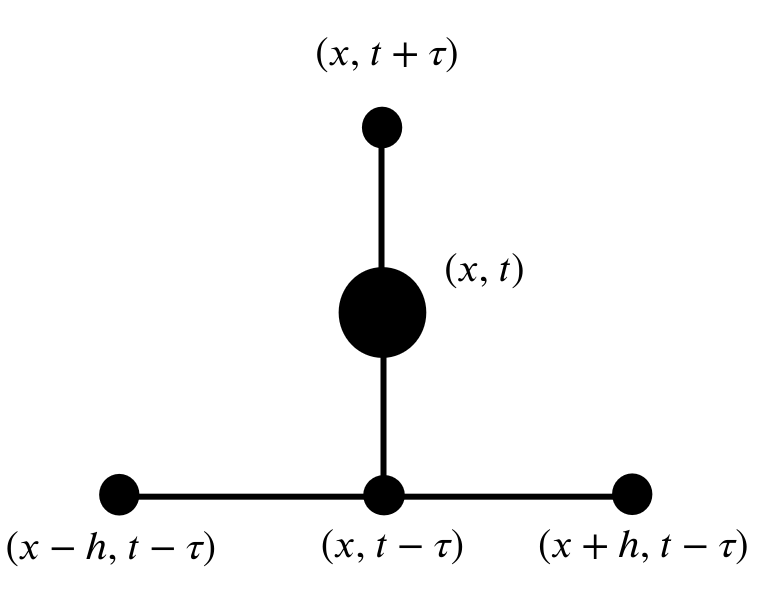
\includegraphics[scale=0.25]{images/img_6}
			$$
			\item Шаблон может иметь вид 
			$$
				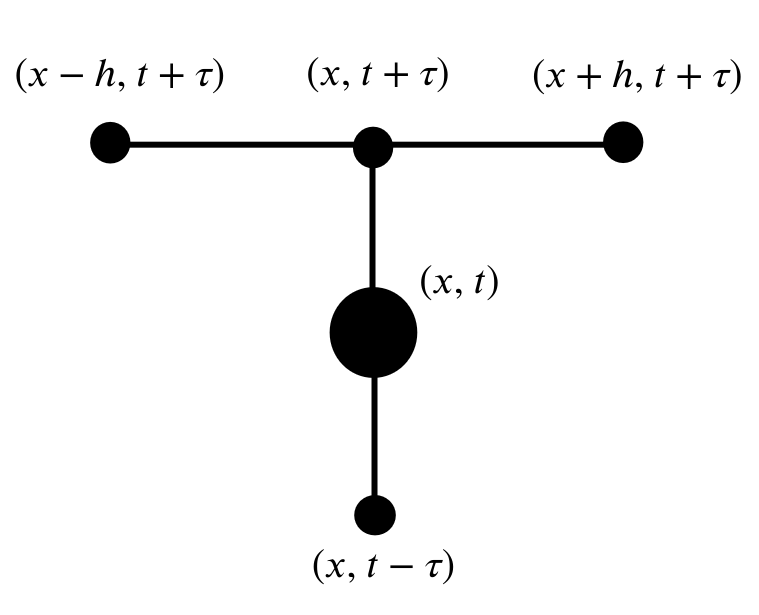
\includegraphics[scale=0.25]{images/img_7}
			$$
			\item Шаблон может иметь вид $$
				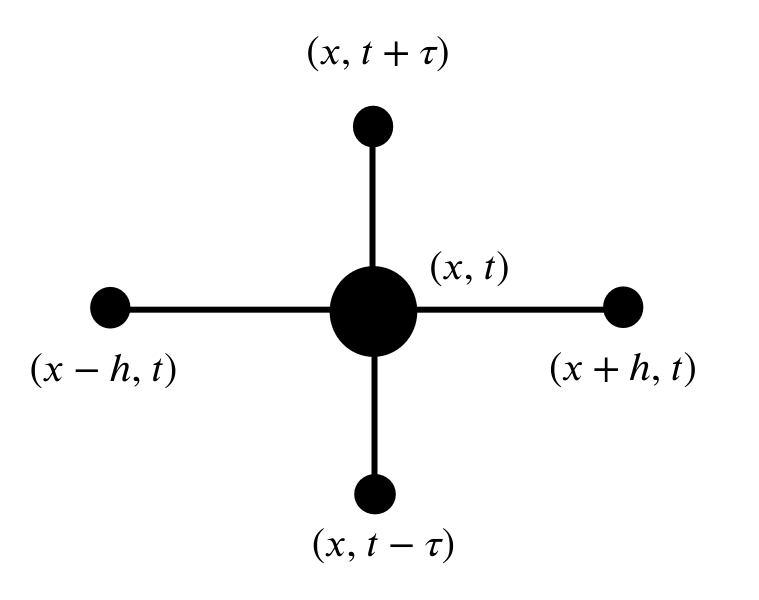
\includegraphics[scale=0.25]{images/img_8}
			$$
			\item Шаблон может иметь вид 
			$$
				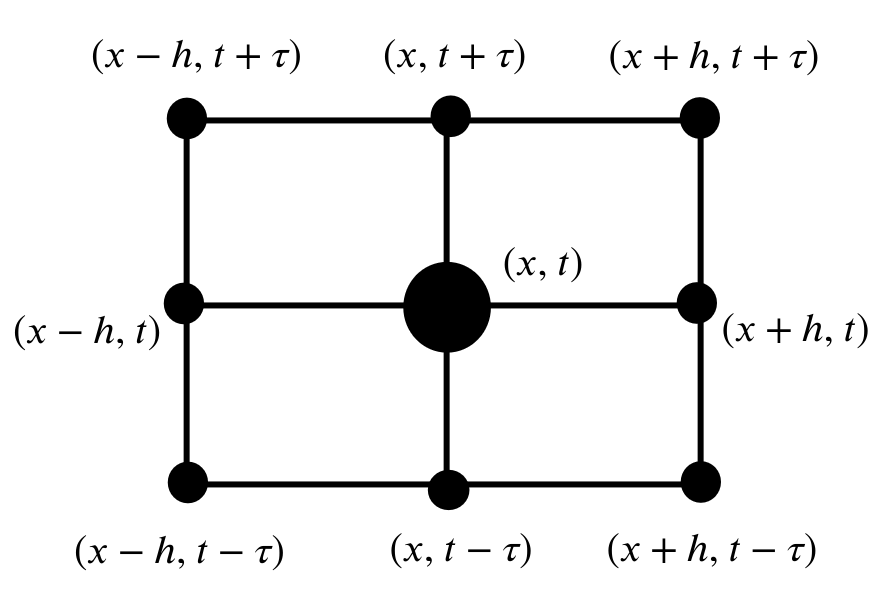
\includegraphics[scale=0.25]{images/img_9}
				$$
		\end{enumerate}
		Запишем двухпараметрическое семейство для варианта (d)
		\begin{equation}
			L_{h\tau}^{(\sigma_1, \sigma_2)}u = u_{\ol t t} - (\sigma_1 \hat u_{\ol x x} + (1-\sigma_1 - \sigma _2) u_{\ol x x} + \sigma_2 \check u_{\ol x x}).
		\end{equation}
		Для шаблона (а) \begin{equation}
			L_{h\tau}^{(0,1)} u= u_{\ol t t} - \check u_{\ol x x}.
		\end{equation}
		Для шаблона (b) \begin{equation}
			L_{h\tau}^{(1,0)} u= u_{\ol t t} - \hat u_{\ol x x}.
		\end{equation}
		Для шаблона (c) \begin{equation}
			L_{h\tau}^{(0,0)} = u_{\ol t t} - u_{\ol x x}.
		\end{equation}
			\end{enumerate}
		Погрешность аппроксимации оператора (14) будет равна $$\psi(x,t) = O(h^2 + \tau^2),\ \sigma_1=\sigma_2 = 0.$$
		Если же $\sigma_1 = \sigma_2 = \sigma$, то погрешность будет также иметь второй порядок
		$$\psi(x,t) = O(h^2 + \tau^2).$$
		Для других значений погрешность аппроксимации по $h$ понижается.
		\subsection{}
		
		\begin{enumerate}
			\item .
			\item Пусть $\omega_h$ одномерно и неравномерно. Тогда $h$ будет определяться набором шагов между каждой точкой $$h = (h_1,\ldots, h_N),$$ где $N$ -- это число разбиений. В данном случае $$|h| = \underset{1\leq i \leq N}{\max}h_i.$$
		\end{enumerate}
		\textbf{Пример 5.} Рассмотрим аппроксимацию оператора $$Lu = u''(x),\ u\in H_0 = C^4[0,1].$$
		Случай, когда сетка равномерная, нас не интересует. Построим на отрезке $[0,1]$ неравномерную сетку $$\hat{\ol \omega_h} = \{x_0 < x_1 < \ldots < x_N,\ x_i = x_{i-1}+h_{i},\ i=\ol{1,N},\ x_0=0, x_N=1\}.$$
		Итак $h = (h_1,\ldots, h_N)$, где $h_i = x_i - x_{i-1},\ i=\ol{1,N}.$ Для каждого $x_i$, $i=\ol {1, N-1}$ рассмотрим трехточечный шаблон $\{x_{i-1}, x_i, x_{i+1}\}$ и методом неопределенных коэффициентов построим разностный оператор \begin{equation}
			(L_hu)_i = \dfrac{1}{ \hbar_i}\left(\dfrac{u(x_{i+1} - u(x_i))}{h_{i+1}} - \dfrac{u(x_i) - u(x_{i-1})}{h_i}\right)u_{\ol x \hat x}.
		\end{equation}
		В формуле (17) $$\hbar_i = \dfrac12 (h_i + h_{i+1}),\ u_{\hat x}=\dfrac{1}{\hbar_i}(u(x_{i+1} - u(x_i))).$$
		Если будем рассматривать погрешность в каждой точке сетки $x_i$, то получим
		$$\psi_i = \dfrac{h_{i+1} - h_i}{3}u''(x_i) + O(\hbar_i^2),\ i = \ol{1, N-1}.$$
		Из этого выражения следует, что в сеточной норме $$\Norm{\cdot}_{h, C} = \underset{x \in \hat \omega_h}{\max}|\cdot |$$
		норма погрешности равна
		$$\Norm{\psi_h}_{h,C} = \underset{1\leq i \leq N}{\max}|\psi_i|=O(h),$$
		где $h = \underset{1\leq i \leq N}{\max}h_i.$
		Но можно подобрать другую норму, в которой порядок аппроксимации будет другим. Рассмотрим другую норму в пространстве сеточных функций -- \textit{негативную норму}
		$$\Norm{\psi_h}_{h, -1}=\sqrt{\sum_{i=1}^{N-1}h_i\left(\sum_{k=1}^i \hbar_k \psi_k\right)^2}.$$
		Тогда можно доказать, что величина погрешности в этой норме равна
		$$\Norm{\psi_h}_{-1} = O(h^2).$$
		Таким образом, локальное условие погрешности может быть недостаточным.
		Выбор подходящей нормы всякий раз должен быть предметом изучения. \\\\
		Рассмотрим основные нормы, которые мы дальше будем использовать в случае функций двух измерений. Рассмотрим функцию двух аргументов $u(x,t)$, $(x,t) \in G$ и наряду с ней сеточную функцию $y(x,t)$, $x \in \omega_h$, $t \in \omega_\tau$, которая определена на сетке $\omega_{h\tau} = \omega_h \times \omega_\tau$. В сеточном пространстве мы будем рассматривать в основном такую норму 
		$$\Norm{y}_{h\tau} = \underset{t \in \omega_h}{\max}\Norm{y(t)}$$
		или 
		$$\Norm{y}_{h\tau} = \sqrt{\sum_{t \in \omega_\tau}\tau \Norm{y(t)}_h^2}.$$
		\textbf{Пример 6.}
		Рассмотрим оператор $$Lu = \dfrac{\d u}{\d t} - \dfrac{\d ^2 u}{\d x ^2},\ u \in H_0 = C^{4,2}[0,1].$$
		Возьмем простейшую аппроксимацию
		$$L_{h\tau}u = u_t - u_{\ol xx}.$$
		Если по $x$ сетка равномерна, то $h$ фиксировано. Распишем оператор в любой точке сетки
		$$L_{h\tau}u = u_t - u_{\ol xx} = \dfrac{u_i^{j+1} - u_i^j}{\tau} - \dfrac{u_{i+1}^j - 2u_i^j + u_{i-1}^j}{h^2}.$$
		В данном случае в качестве сеточной функции $y$ мы рассматриваем проекцию $u$ на сетку, то есть $u=u(x_i, t_j) = u_i^j$.
		Локальная погрешность аппроксимации имеет вид $$L_{h\tau}u - (Lu)_{h\tau} = \psi_{h\tau}(x_i, t_j) = O(\tau + h^2).$$
		Легко показать, что данный разностный оператор аппроксимирует исходный оператор на сетке с первым порядком по $t$ и вторым порядком по $x$ в любой из норм, рассматриваемых выше, то есть 
		$$\Norm{\psi}_{h\tau} = O(\tau + h^2).$$
		Как правило, вычислив погрешность аппроксимации в точке, то она обобщается и на всю сетку.
		\section{Разностная аппроксимация дифференциальных задач.}
		\subsection{Постановка разностной задачи.}
		Как известно, дифференциальная задача включает в себя дифференциальное уравнение и дополнительные условия, которые выделяют из совокупности возможных решений единственное. Поэтому при формулировке разностных задач помимо аппроксимации дифференциальных уравнений, необходимо описывать в разностных уравнениях и дополнительные условия.\\\\
		$\bullet$ \textit{Совокупность разностных уравнений, аппроксимирующих дифференциальное уравнение и дополнительные условия, называется \textbf{разностной схемой}.}\\\\
		$\bullet$ \textit{Существуют две формы записи разностных схем: \textbf{безындексная} и \textbf{индексная}.}\\\\
		\textbf{Пример 1.} Рассмотрим задачу вида 
		\begin{equation}
			\begin{cases}
			u'(t) = f(t),\ t>0,\\
		u(0) = u_0 = \const.
		\end{cases}
		\end{equation}
		Для того, чтобы построить разностную схему, необходимо выписать разностное уравнение, которое будет аппроксимировать исходное дифференциальное уравнение. Для начала построим равномерную сетку $$\omega_\tau = \{t_j = j\tau,\ \tau>0,\ j=0,1,\ldots\}.$$
		Тогда дифференциальной задаче можно поставить в соответствие разностную схему в \textit{безындексной форме}
		\begin{equation}
			\begin{cases}
			y_t = \varphi,\ t \in \omega _t,\\
			y(0) = u_0,
		\end{cases}
		\end{equation}
		или в \textit{индексной форме}
		\begin{equation}
			\begin{cases}
				\dfrac{y^{j+1}-y^j}{\tau} = \varphi^i,\ j=0,1,\ldots,\\
				y(0) = u_0,
			\end{cases}
		\end{equation}
		при этом $$y^j = y(t_j)\approx u(t_j),\ \varphi^j = \varphi(t_j).$$
		При этом права часть в разностном уравнении может быть задана различными способами, но при условии выполнения следующего соотношения -- \textit{необходимого условия для обеспечения первого порядка аппроксимации}
		$$\varphi - f = O(\tau).$$
		Например, в качестве $\varphi$ можно выбирать и $\varphi(t) = f(t)$, $t \in \omega_{\tau}$. Также можно выбирать $$\varphi(t) = \dfrac{f(t) + f(t+\tau)}{2}.$$
		После записи разностной схемы необходимо указать способ реализации этой схемы.\\\\ $\bullet$ \textit{\textbf{Под способом реализации} будем понимать построение вычислительного алгоритма, позволяющий найти приближенное решение во всех узлах сетки.}\\\\
		В нашем примере способ реализации тривиален. Для способа реализации используется, как правило, индексная форма записи. Запишем алгоритм реализации разностной схемы (2)-(3)
		\begin{equation}
			y^{j+1}=y^j + \tau \varphi^j,\ j=0,1,\ldots,\ y^0 = u_0.
		\end{equation}
		Таким образом, для дифференциальной задачи (1) разностная схема (2)-(3) позволяет найти приближенное решение по алгоритму ее реализации (4).
		\\\\
		\textbf{Пример 2.}
		Рассмотрим задачу для функции двух переменных для уравнения гиперболического типа
		\begin{equation}
			\begin{cases}
				Lu = f(x,t), \ L = \dfrac{\d }{\d t} - \dfrac{\d ^2}{\d x^2},\\
			u = u(x,t),\ 0<x<1,\ 0<t<T,\\
			u(x,0) = u_0(x), \ 0\leq x \leq 1,
			u(0,t) = \mu_0(t),\ u(1,t) = \mu_1(t),\ 0\leq t\leq T.
			\end{cases}
		\end{equation}
		Для аппроксимации задачи сперва мы должны выписать разностные уравнения, которые определяются приближением соответствующих разностных операторов и заменой непрерывной функции на сеточный аналог. Для простоты построим равномерную по $h$ и $\tau$ сетку узлов
		$$\ol \omega_{h\tau} = \ol \omega_h \times \ol \omega_\tau.$$
		Выберем шаблон
		$$\text{Ш}(x,t) = \{(x-h, t),\ (x,t),\ (x+h,t),\ (x,t+\tau)\},\ x\in \omega_h,\ t \in \omega_\tau.$$
		Вместо исходной задачи (5) получим разностную задачу, которая и будет являться разностной схемой в \textit{безындексной форме записи}
		\begin{equation}
			\begin{cases}
				y_t = y_{\ol x x} + \varphi,\ \varphi = f+O(\tau + h^2),\ (x,t)\in \omega_{h\tau},\\
			y(x,0) = u_0(x),\ x\in \ol \omega_h,\\
			y(0, t) = \mu_0(t),\ y(1,t) = \mu_1(t),\ t\in \ol\omega_\tau.
			\end{cases}
		\end{equation}
		Запишем сразу алгоритм реализации этой разностной схемы:
		\begin{equation}
			\begin{cases}
			y_i^{j+1} = y_i^j + \tau \left(\dfrac{y_{i+1}^j - 2y_i^j + y_{i-1}^j}{h^2} + \varphi_i^j\right),\ i=\ol{1, N_x-1},\ j=\ol{1, N_t-1},\\
		y_i^0 = u_0(x_i),\ i=\ol{0,N_x},\\
		y_0^j = \mu_0(t_j),\ y_{N_x}^j = \mu_1(t),\ j=\ol{1, N_t}
		\end{cases}
		\end{equation}
		\subsection{Сходимость и точность разностных схем.}
		Пусть дана дифференциальная задача 
		\begin{equation}
			Lu = f(x),\ x \in G,
		\end{equation}
		\begin{equation}
			lu = \mu(x),\ x \in \Gamma.
		\end{equation}
		Искомая функция $u(x) \in H_0$, $x \in \ol G = G \cup \Gamma$, а $L$, $l$ -- дифференциальные операторы, действующие в пространстве $H_0$ c нормой $\Norm{\cdot}_0$.
		Задаче (8)-(9) на сетке $\ol\omega_h = \omega_h \cup \gamma_h$ поставим в соответствие разностную задачу, или разностную схему
		\begin{equation}
			L_h y_h = \varphi_h,\ x \in \omega_h
		\end{equation}
		\begin{equation}
			l_h y_h = \chi _h,\ x \in \gamma_h
		\end{equation}
		где приближенное решение $y_h(x) \in H_h$, $x \in \ol\omega_h$, а $L_h, l_h$ -- это разностные операторы, дествующие в пространстве $H_h$ с нормой, которая согласована с нормой пространства $H_0$, то есть
		$$\lim\limits_{h \to 0}\Norm{\cdot}_h = \Norm{\cdot}_0.$$
		$\bullet$ \textit{Разностная задача должна быть \textbf{корректно поставленной}, то есть}
			\begin{enumerate}
				\item решение $y_h(x)$ задачи $(10)-(11)$ существует и единственно для всех $\varphi_h$, $\chi_h$ из допустимого семейства сеточных функций;
				\item решение $y_h(x)$ непрерывно зависит от $\varphi_h$, $\chi_h$, то есть для любого шага сетки $h_0$ существует константа $M$ такая, что при всех $h \leq h_0$ выполняется неравенство $$\Norm{y_h-\widetilde{y}_h}_h \leq M\left(\Norm{\varphi_h - \widetilde{\varphi}_h}_h + \Norm{\chi_h - \widetilde{\chi}_h}_h\right),$$
				где $\widetilde{y}_h$ -- решение задачи (11) с правыми частями $\widehat{\varphi}_h$, $\widehat{\chi}_h$. Непрерывная зависимость решений разностной задачи называется \textbf{устойчивостью по входным данным}.
			\end{enumerate} 
			Факт наличия устойчисовсти является одним из основных вопросов теории разностных схем.\\\\
			Основной целью всякого приближенного метолда является получения решения исходной непрерывной задачи с заданной точностью $\epsilon$ за конечное число ействий $k$. Поэтому после построения разностной схемы, аппроксимирующей исходную задачу, мы должны убедиться в том, что решение разностной задачи $y_h$ будет являться приближенным значением точного решения задачи $u(x)$.\\\\
			Пусть $u_h$  -- это значения исходной функции $u(x)$ на сетке $\omega_h$. Рассмотрим погрешность разностной схемы (10)-(11). Для этого введем функцию $$z_h = u_h - y_h.$$ Выразим $y_h = u_h - z_h$ и подставим в задачу (10)-(11). Тогда получим задачу для погрешности 
			\begin{equation}
			L_h z_H = \psi_h,\ x \in \omega_h,
			\end{equation}
			\begin{equation}
				l_h z_h = \nu_h,\ x \in \gamma_h,
			\end{equation}
			где
			$$\psi_h = L_h u_h - \varphi_h$$
			$$\nu_h = l_hu_h - \chi_h.$$
			\textit{$\bullet$ Функция $\psi_h$ называтеся \textbf{погрешностью аппроксимации уравнения (8) разностным уравнением (10)}. А функция $\nu_h$ -- \textbf{погрешностью аппроксимации граничныз условий (9) разностными условиями (11)}.}\\\\
			Для оценки погрешности $z_h$ и погрешность аппроксимации введем на сеточном множестве функций нормы $\Norm{\cdot}_{1,h}$, $\Norm{\cdot}_{2,h}$, $\Norm{\cdot}_{3,h}$.\\\\
			$\bullet$ \textit{Будем говорить, что решение разностной задачи (10)-(11) сходится к решению непрерывной задачи (1)-(2) (что то же самое \textbf{разностная схема (10)-(11) сходится}), если }
			\begin{equation}
				\Norm{z_h}_{1,n}= \Norm{u_h - y_h}_{1,h} \xrightarrow[|h| \to 0]{}0.
			\end{equation}
			\textit{Разностная схема имеет $n$-ый порядок точности, если при достаточно малом $|h|\leq |h_0|$ выполняется неравенство}
			\begin{equation}
				\Norm{z_h}_{1,n}\leq M|h|,
			\end{equation}
			\textit{где $M$ -- константа, не зависящая от $h>0$.}
			Р\textit{азностная схема имеет $m$-ый порядок аппроксимации, если} \begin{equation}
				\Norm{\psi_h}_{2,h} = O(|h|^m),\ \Norm{\nu_h}_{3,h} = O(|h|^m).
			\end{equation}
			Обозначим через $f_h$ и $(Lu)_h$ значения правой части уравнения (8) на сетке и значение $Lu$ на сетке. С учетом того, что 
			$$(Lu - f)_h = 0,$$
			то можно погрешность аппроксимации уравнения записать в виде
			$$\psi_h = \psi_h^{(1)} + \psi_h^{(2)},$$
			где
			$$\psi_h^{(1)} = f_h - \varphi_h,$$ -- погрешнрсть аппроксимации правой части
			$$\psi_h^{(1)} = L_h u_h - (Lu)_h,$$ -- погрешность аппроксмации дифференциального оператора. Аналогично можно записать и для $\nu_h$.\\\\
			Оказывается, что понятия сходимости и точности связаны между собой для линейных разностных схем. Зависимость порядка точности от порядка аппроксимации дает теорема Лакса.
			\begin{theorem}
				[Лакса] Если линейная разностная схема устойчива и аппроксимирует исходную дифференциальную задачу, то она сходится. Причем порядок точности схемы определяется порядком ее аппроксимации.
			\end{theorem}
			\subsection{Повышения порядка аппроксимации разностных схем.}
			Поскольку порядок сходимости разностной схемы, а значит и скорость сходимости приближенного решения к точному зависит от порядка аппроксимации, то вопрос об увеличении порядка аппроксимации без увеличения геометрического шаблона является весьма важным для исследования разностных схем.
			\\\\
			\textbf{Пример 3.} Возьмем задачу и разностную схему из примера 1.
			Рассмотрим погрешность аппроксимации 
			\begin{multline*}
				\psi_\tau(t) = u_t(t) - \varphi(t)= \dfrac{u(t_\tau) - u(t)}{\tau} - \varphi(t) = \left[u(t+\tau) = u(t)+\tau u'(t) + \dfrac{\tau^2}{2}u''(t) + O(\tau^3)\right]=\\ = [u'(t) = f(t),\ u''(t) = f'(t)]=f(t) + \dfrac\tau2 f'(t) - \varphi(t) + O(\tau^2)
			\end{multline*}
			Можно в самом простом случае выбрать $$\varphi(t) = f(t) + O(\tau).$$ Тогда мы получим разностную схему первого порядка $\psi_\tau = O(\tau).$ Причем при таком выборе $\varphi = f$ мы получили \textit{явный метод Эйлера}.\\\\
			Мы также можем взять $$\varphi(t) = f(t) + \dfrac \tau 2 f'(t) + O(\tau^2).$$
			Тогда, если мы возьмем
			$$\varphi = f\left(t + \dfrac\tau2\right),$$
			то из $\varphi(t)$ аппроксимирует выражение выше с порядком $O(\tau^2)$. Подставив это в нашу разностную схему, мы получим схему второго порядка аппроксимации. А это есть ничто иное, как \textit{формула средних прямоугольников}.\\\\
			В качестве $\varphi$ можно выбирать и другие выражения. Например, если выбирать
			$$\varphi = f(t) + \dfrac\tau2 f_t(t),$$ то мы получим \textit{формулу трапеций}.\\\\
			Мы повышали порядок аппроксимации исходя из выбора правой части основного уравнения. Но чаще всего получается так, что задача задается с такими граничными условиями, в которых при минимальном шаблоне понижается порядок аппроксимации. Рассмотрим такой случай
			\\\\
			\textbf{Пример 4.} Рассмотрим третью краевую задачу для обыкновенного дифференциального уравнения следующего вида
			\begin{eqnarray}
					u''(x) - qu(x) = f'(x),\ 0<x<1,\\
					u'(0) = \sigma_0 u(0) - \mu_0,\\
					u(1) = \mu_1
			\end{eqnarray}
			В уравнениях (18)-(20) числа $q, \sigma_0, \mu_0, \mu_1$ -- это заданные константы. Построим равномерную сетку $\ol \omega_h = \omega_h \cup \gamma_h$ на отрезке $[0,1]$, где
			$$\omega_h = \left\{x_i = ih,\ i = \ol {1,N-1}, h = \dfrac1N\right\},$$
			$$\gamma_h = $$
			Для аппроксимации уравнения (18) выберем шаблон $$\text{Ш}_1(x) = \{x-h, x, x+h\},\ x \in \omega_h.$$
			Для аппроксимации условия (19) выберем шаблон, состоящий из двух точек
			$$\text{Ш}(0) = \{x_0, x_1\} = \{0,h\},$$
			Для аппроксимации условия (20) формально выбираем шаблон
			$$\text{Ш}_3(1) = \{x_N\} = \{1\}.$$
			Заменяем дифференциальные производные разностными и строим разностную схему
			\begin{eqnarray}
				y_{\ol x x}(x) - dy(x) = -\varphi(x),\ x\in \omega_h,\\
				y_x(0) = \sigma_0 y(0) - \mu_0,\\
				y(1) = \mu_1.
			\end{eqnarray}
			Исследуем погрешность аппроксимации. Для любого узла $x \in \omega_h$ запишем величину погрешность как невязку над точным решением
			$$\psi_h = u_{\ol x x} - du + \varphi.$$
			Воспользуемся соотношениями
			$$u_{\ol x x} = u'' + \dfrac{h^2}{12}u^{(IV)} + O(h^4).$$
			Учитывая, что $u'' = qu - f$, получим
			$$\psi_h = qu - f + \dfrac{h^2}{12}u^{(IV)} - du + \varphi + O(h^4) = (q-d)u + (\varphi - f) + O(h^2).$$
			Отсюда видно, что $\psi_h = O(h^2)$, если мы выберем
			$$d = q+ O(h^2),\ \varphi = f + O(h^2),$$ то разностное уравнение (21) будет аппроксимировать исходное разностное уравнение со вторым порядком. \\\\
			Рассмотрим погрешность аппроксимации граничных условий
			\begin{multline*}
				\nu_h(0) = u_x(0) - \sigma_0 u(0) + \mu_0 = u'(0) + \dfrac h2 u''(0) + O(h^2) - \sigma_0 u(0) + \mu_0 =\\= [u'(0) =\sigma_0 u(0) - \mu_0] = \dfrac{h}{2}u''(0) + O(h^2) = O(h).
			\end{multline*}
			Исследуем аппроксимацию второго граничного условия
			$$\nu_h(1) = u(1) - \mu_1 = 0,$$
			то есть условие аппроксимируется точно.\\\\
			В итоге мы получили погрешность аппроксимации граничных условий
			$$\nu_h = \nu_h(0) + \nu_h(1) = O(h),$$ поэтому общий порядок аппроксимации равен сумме порядков аппроксимации
			$$\Psi = \psi_h + \nu_h = O(h).$$
			Следовательно, мы построили схему первого порядка аппроксимации.\\\\
			В данном случае возникает потребность повысить порядок точности схемы, не изменяя размер шаблона. Для этого нам необходимо повысить порядок $\nu_h(0)$. Чтобы добиться этого, введем вместо коэффициентов $\sigma_0$ и $\mu_0$ сеточные коэффициенты $\ol \sigma_0, \ol \mu _0$. Тогда вместо уравнения (22) будем рассматривать уравнение с этими коэффициентами
			\begin{equation}
				y_x(0) = \ol \sigma_0 + \ol \mu _0
			\end{equation}
			 и подберем эти коэффициенты так, чтобы погрешность аппроксимации была равна $O(h^2)$. Выписываем погрешность аппроксимации с новыми коэффициентами, предполагая, что исходное дифференциальное уравнение (18) выполняется в точке $x =0$.
			 \begin{multline*}
			 	\nu_h(0) = u_x(0) - \ol\sigma_0 u(0) + \ol\mu_0 = u'(0) - (\ol\sigma_0 u(0) - \ol \mu_0)+ \dfrac h2 u''(0) + O(h^2) =\\= [u''(0) =qu(0) - f(0),\ u'(0)=\sigma_0 u(0) - \mu_0] =\\= \left[\left(\sigma_0 + \dfrac h2 q\right) - \ol\sigma_0\right]u(0) + \left[\ol \mu_0 - \left(\mu_0 + \dfrac h2 f(0)\right)\right] + O(h^2)
			 \end{multline*}
			 Если мы выберем
			 $$\ol \sigma = \sigma_0 + \dfrac h2 q,\ \ol\mu_0 = \mu_0 + \dfrac h2 f(0),$$ то в уравнении (24) мы получим второй порядок аппроксимации, а значит схема (21), (24), (23) будет являться схемой второго порядка аппроксимации.\\\\
			$\bullet$ \textit{Такой способ повышения порядка аппроксимации назвыается \textbf{методом повышения порядка с использованием вида дифференциального оператора}.}
	\end{document}
	
	


	